\documentclass[12pt,a4paper]{article}

\usepackage[utf8]{inputenc}
\usepackage[russian]{babel}
\usepackage[OT1]{fontenc}
\usepackage{amsmath}
\usepackage{amsfonts}
\usepackage{amssymb}
\usepackage{makeidx}
\usepackage{graphicx}
\usepackage[left=2cm,right=2cm,top=2cm,bottom=2cm]{geometry}

\author{Николай Анохин}

\begin{document}

\subsection*{Задача 1}

Пусть имеется информация о покупках, совершаемых 100 миллионами людей, каждый из которых ходит в магазин в среднем 100 раз в году и покупает 10 из 1000 предложенных товаров. Предположим, что два человека попадают под подозрение, если они купили в течение года в точности один и тот же набор товаров (возможно, для изготовления бомбы?). С помощью принципа Бонферрони определите, будет ли эффективным метод выявления террористов, основанный на поиске таких пар людей.

\subsection*{Задача 2}

На рисунке показан набор из $9$ точек, расположенных на плоскости. Примените алгоритм иерархической кластеризации с single-link расстоянием между кластерами. Постройте дендрограмму.
\begin{center}
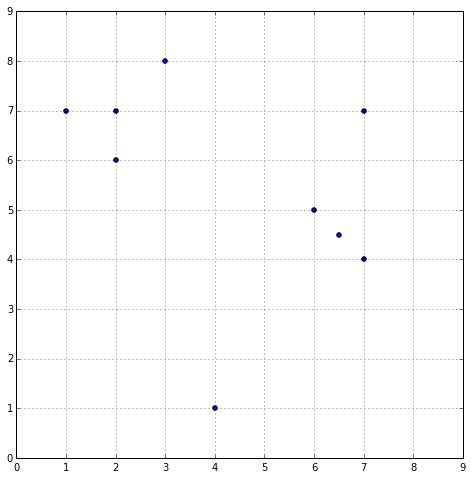
\includegraphics[scale=0.5]{2.png}
\end{center}
Какова алгоритмическая сложность этого алгоритма?

\subsection*{Задача 3}

В таблице даны попарные расстояния между объектами из обучающей выборки. Проведите иерархическую кластеризацию с использованием complete-link расстояния между кластерами.

\begin{center}
\begin{tabular}{l | c c c c c c}
 & $x_1$ & $x_2$ & $x_3$ & $x_4$ & $x_5$ & $x_6$ \\
\hline
$x_1$ & $0.0$ & $1.5$ & $5.0$ & $4.0$ & $2.5$ & $0.5$ \\
$x_2$ & & $0.0$ & $4.0$ & $0.5$ & $3.5$ & $2.0$ \\
$x_3$ & & & $0.0$ & $6.0$ & $2.0$ & $1.0$ \\
$x_4$ & & & & $0.0$ & $5.5$ & $4.5$ \\
$x_5$ & & & & & $0.0$ & $1.0$ \\
$x_6$ & & & & & & $0.0$ \\
\end{tabular}
\end{center}

\subsection*{Задача 4}

Пусть алгоритм, кластеризуюзщий точки в многомерном Евклидовом пространстве, оптимизирует критерий ($k$ задано)
\[
J = \frac{1}{2}\sum_{k} \sum_{x_i \in C_k} \sum_{x_j \in C_k} \| x_i - x_j \|^2.
\]
Покажите, что такой алгоритм эквивалентен стандартному алгоритму k-means.

\subsection*{Задача 5}

Пусть даны 2 кластеризации $C$ и $\Omega$ одного и того же набора данных. Покажите, что
\[
MI(C, \Omega) \leq \frac{1}{2} (H(C) + H(\Omega)),
\]
где $MI(C, \Omega)$ -- mutual information, а $H(C)$ и $H(\Omega)$ -- соответствующие энтропии.

\subsection*{Задача 6}

Пусть дана обучающая выборка $X_N$, которая сгенерирована из распределения Стьюдента с неизвестными параметрами $\mu$  и $\sigma$ и известным количеством степеней свободы $\nu$. Используя принцип максимального правдоподобия, получите оценки для неизвестных параметров $\mu$ и $\sigma$.

\subsection*{Задача 7}

Рассмотрим задачу, в которой в качестве объектов рассматриваются строки, а расстояние между объектами -- расстояние правок (edit distance). Существует как минимум два способа выбора центроида (clustroid) в такой задаче: 
\begin{enumerate}
\item выбирать объект, сумма расстояний от которого до всех остальных минимальна;
\item выбирать объект, максимальное расстояние от которого до всех остальных минимально;
\end{enumerate}
Приведите пример кластера, для которого эти варианты дают разные центроиды.

\end{document}